\documentclass[a4paper,titlepage,11pt]{article}

\usepackage[utf8x]{inputenc}
\usepackage{graphicx}

\begin{document}

\begin{titlepage}
\begin{center}
  {\scshape \huge Project Title \par}                                                                         % TODO change the title
  \vspace{1cm}

  {\scshape \LARGE Proposal \par}
  \vspace{1.5cm}

  {\scshape \Large Network and Computer Security \par}
  \vspace{0.5cm}

  {\Large Alameda \par}
  \vfill

  {\itshape \Large Group 11 \par}
  \vfill

\begin{tabular}{l l l}
  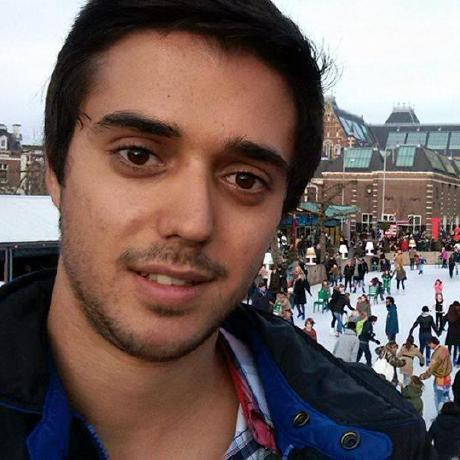
\includegraphics[width=10mm, height=10mm]{img/bernardo.jpeg} & Bernardo Casaleiro & 87827\\
  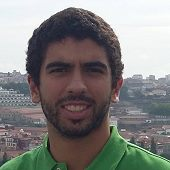
\includegraphics[width=10mm, height=10mm]{img/joao.jpeg} & João Godinho & 87830\\                       % TODO change the photo
  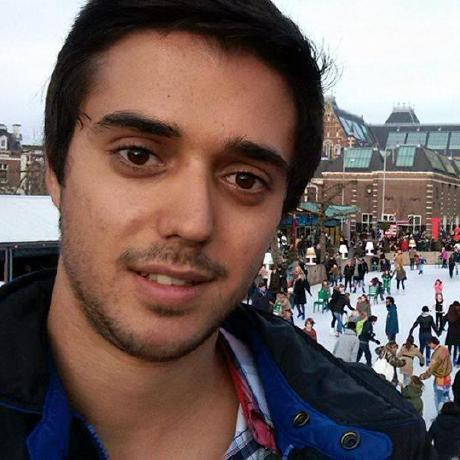
\includegraphics[width=10mm, height=10mm]{img/bernardo.jpeg} & Miguel Pinto & nnnnn\\                       % TODO change the photo and student number
\end{tabular}
  \vfill

  {\large \today\par}
\end{center}
\end{titlepage}

\section{Problem}

\section{Requirements}
	\subsection{Application Requirements}
		\begin{enumerate}
			\item User must be able to send a request of an emergency, that includes id, location and situation

			\item User will be inserted on a queue depending on his rating
			
			\item The server must send a notification to the user, telling the expected time to be answered. 

			\item The server must receive the request and save it on a database and on the log

			\item The server must send the confirmation that an ambulance is en route 

			\item The server must rate the user at the end of the request

			\item The server must be able to block a user from sending more requests (REVIEW)

			
			

 
		\end{enumerate}

	\subsection{Functional Security Requirements}
		\begin{enumerate}
			\item Non-repudiation using certification
			
			\item Keeping the server running in case of DoS
			
			\item There will be a firewall, responsible for filtering the requests

			\item Auditing mechanisms will be implemented

			\item Establish a secure channel between user and Dispatch Central

		\end{enumerate}
	\subsection{Non-Functional Security Requirements}
			Our main goal is to build a secure application, not forgetting that in real life, our service couldn't be slow due to the fact that time in an emergency situation is crucial.


\section{Proposed solution}

\section{Tool references}

\section{Work Plan}

\end{document}
